\chapter{Experimental Setup and Results}

In this chapter, I will describe our experimental setup and results. It includes a breif discussion of our optical tables setup (\ref{exp:laser-table} and \ref{exp:machine-table}), the implementation, optimization and performance of each steps (\ref{exp:zeeman}, \ref{exp:mot}, \ref{exp:gm}, \ref{exp:pump}, \ref{exp:mt} and \ref{exp:odt}) and finally some basic characteristic of our BEC (\ref{exp:bec}).

\section{Laser System}\label{exp:laser-table}
The laser table is where we prepare all the light resonance with the Lithium-$7$ transition ($\approx671nm$). As discussed in the previous chapter, there are four distinct lines that we need in the experiment, the combination of $D1$, $D2$ with $F1$, $F2$. At a certain time, we need either $D1$ or $D2$ light with the probability of using both $F1$ and $F2$ at the same time and the laser table is designed to do just this.\\
\begin{figure}
  \begin{center}
    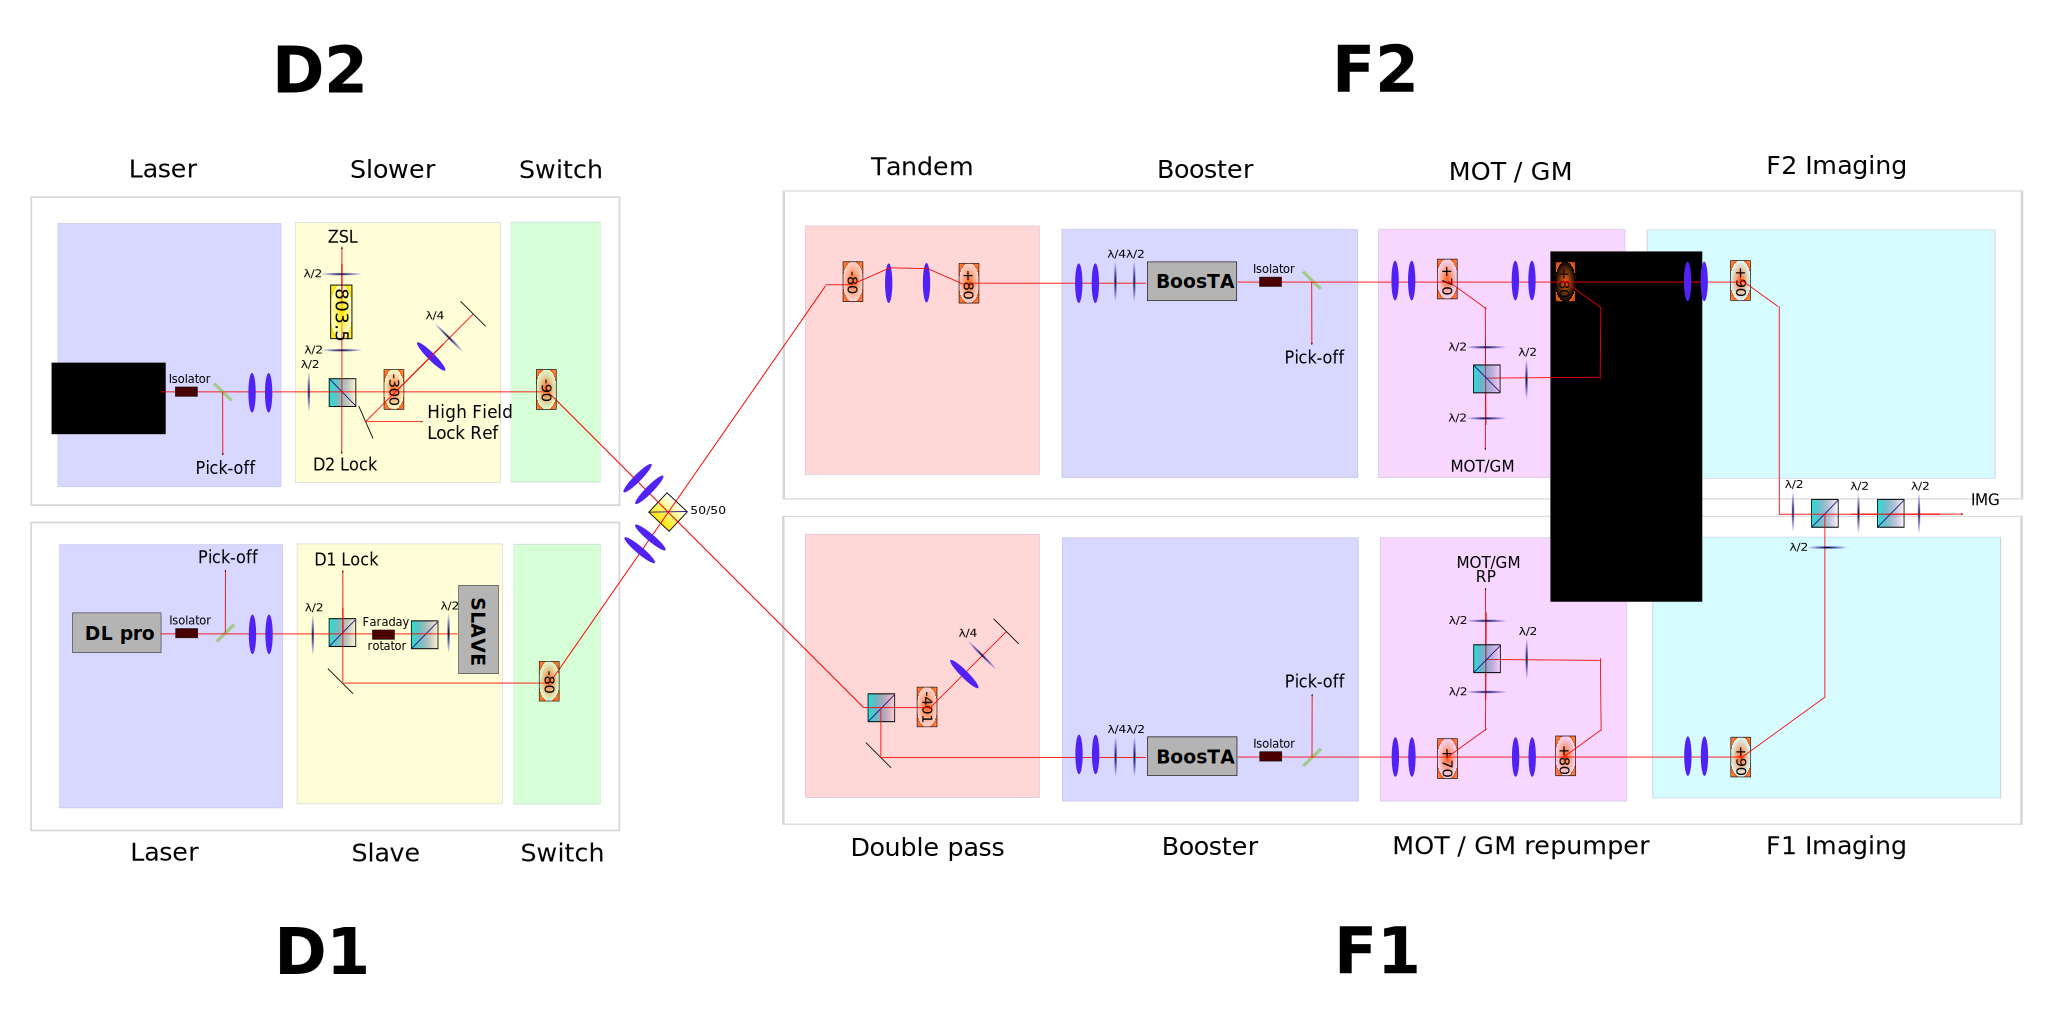
\includegraphics[width=14cm]{laser_table.png}
  \end{center}
  \caption{Schematic of the laser table design}
  \label{exp:laser-table-design}
\end{figure}\\
As shown in figure \ref{exp:laser-table-design}, since the separation between the $D1$ and $D2$ line ($\approx10GHz$) is larger than the range of common optical frequency shifters (e.g. AOM's), the $D1$ and $D2$ light are created separately using two diode lasers (TA pro and DL pro in figure \ref{exp:laser-table-design}). Both of these lasers are actively locked to the appropriate atomic transitions using saturated absorption spectroscopy to better than $2\text{MHz}$. For the $D2$ path, part of the light ($\approx80mW$) is red shifted and used as the Zeeman slower light ($ZSL$ in the figure) and the rest goes to the $D2$, $D1$ selecting switch, which uses two AOMs (acousto-optical modulator) and a $50$-$50$ cube to feed both the $F1$ and $F2$ path with either $D1$ and $D2$ light. For the $D1$ path, a slave diode is used to amplify the light before going to the switch.\\
\\
In the $F1$, $F2$ path, a tandem and a double pass are used to continiously shift the frequency of the laser (the double pass is also used to shift the light from $F2$ to $F1$). After that, the light in each path is amplified using tapered amplifier and then go through a polarization switch consists of two AOMs and a polarization beam splitter which can but the light into polarization maintaining fibers (MOT/GM and MOT/GM RP) with two orthogonal linear polarizations (the use of these beams is further described in section \ref{exp:mot-cage}). At the end of the chain, two more AOMs are used to control the light we put into the imaging fiber so that we can image on any of the four transitions. Each fibers also has a mechanical shutter that se used to block any possible leaking light that may cause heating.

\section{Vacuum Chamber and Main Coils Configuration}\label{exp:machine-table}

\subsection{MOT-Gray Molasses Cage}\label{exp:mot-cage}

\section{Spin Flip Zeeman Slower}\label{exp:zeeman}

\section{Magneto-Optical Trap (MOT) and Compressed-MOT}\label{exp:mot}

CMOT

\section{Gray Molasses}\label{exp:gm}

\section{Dark State Pumping}\label{exp:pump}

At the end of Laser cooling, the atoms are distributed in different ground states.\\
In order to trap in MT, need to go to 2, 2 / 2, 1 which are the only trappable states at both low field and high field.\\
Choose 2, 2 because we can use dark state pumping which ...

Dark State pumping with D1 light

Re-scattering, detuning

\section{Static Magnetic Trap}\label{exp:mt}

\section{Optical Dipole Trap}\label{exp:odt}

\section{Bose-Einstein Condensate}\label{exp:bec}
